
\subsection*{Pictures and Explanation}

%%%Insert this to get the typewriter font so it looks like a real movie script
{\ttfamily
\fontdimen2\font=0.4em
\fontdimen3\font=0.2em
\fontdimen4\font=0.1em
\fontdimen7\font=0.1em
\hyphenchar\font=`\-


%%%%put a hypertarget around the opening bit of text
\hypertarget{solution_sets_for_systems_of_linear_equations_overview}{This video considers solutions sets}
for linear systems with three unknowns. These are often called $(x,y,z)$ and label points in ${\mathbb R}^3$.
Lets work case by case:

\begin{itemize}
\item If you have no equations at all, then any $(x,y,z)$ is a solution, so the solution set is  all of~${\mathbb R}^3$.
The picture looks a little silly:
\begin{center}
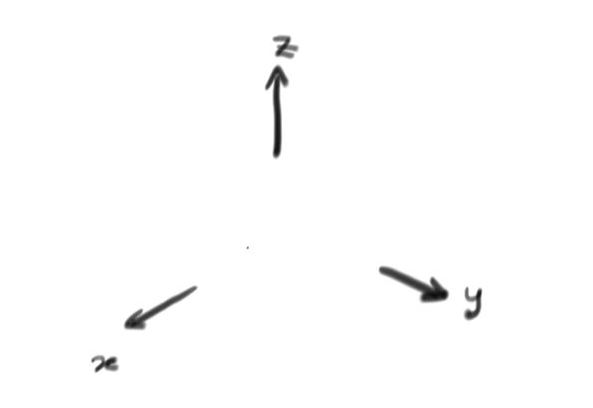
\includegraphics[scale=.15]{all_of_R3.jpg}
\end{center}
\item For a single equation, the solution is a plane. This is explained in this \href{\videourl solution_sets_for_systems_of_linear_equations_planes.mp4}{video}
or the accompanying \hyperlink{solution_sets_for_systems_of_linear_equations_planes}{script}. The picture looks like this:
\begin{center}
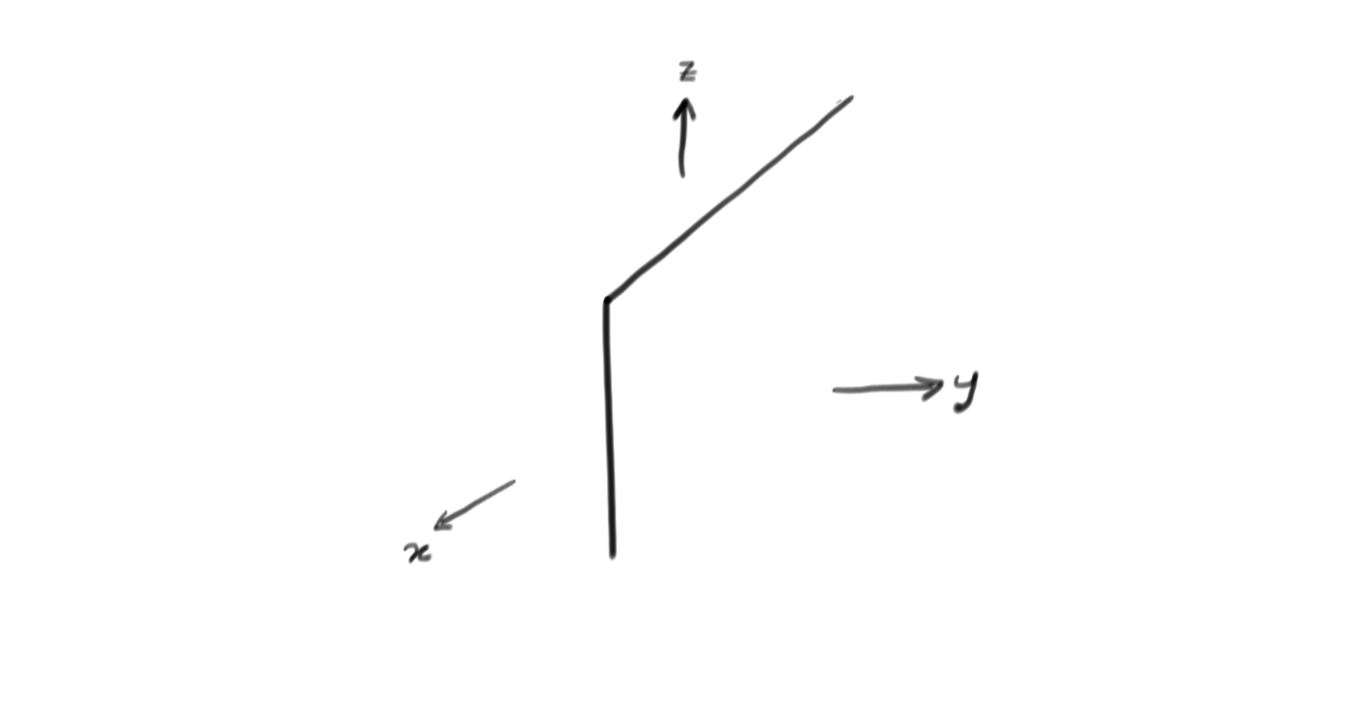
\includegraphics[scale=.18]{plane_in_R3.jpg}
\end{center}
\item For two equations, we must look at two planes. These usually intersect along a line, so the solution set will also (usually) be a line:~\begin{center}
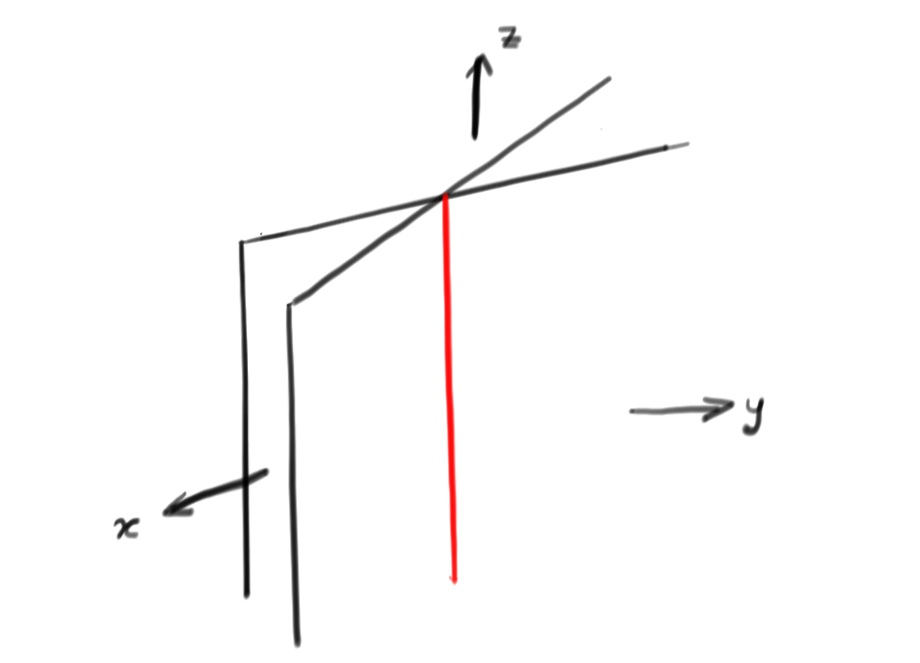
\includegraphics[scale=.18]{two_planes_in_R3.jpg}
\end{center}
\item For three equations, most often their intersection will be a single point so the solution will then be unique:
\begin{center}
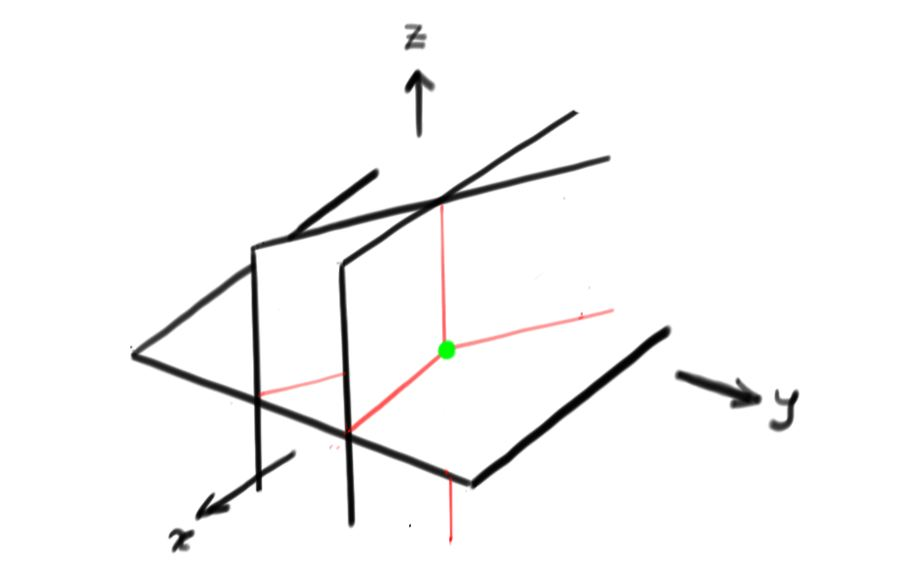
\includegraphics[scale=.17]{three_planes_in_R3.jpg}
\end{center}
\item Of course stuff can go wrong. Two different looking equations could determine the same plane, or worse equations could be inconsistent.
If the equations are inconsistent, there will be no solutions at all. For example, if you had four equations determining four parallel planes the solution set would be empty. This looks like this:
\begin{center}
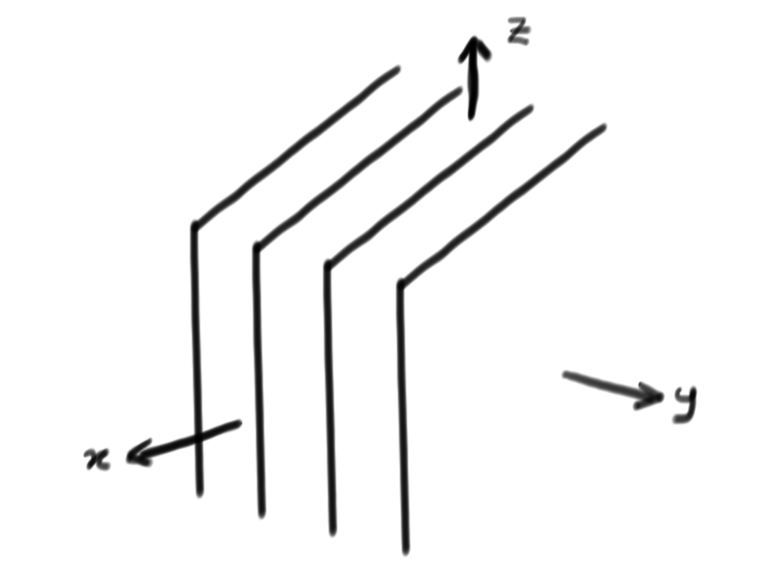
\includegraphics[scale=.16]{four_planes_in_R3.jpg}
\end{center}
\end{itemize}



%%%%don't forget to close the bracket so the stuff after your file doesn't look like a movie!
}

%\newpage
